\newpage
\section{Getting started - Your first solar cell simulation}
No matter which type of device you want to simulate, if you are new to gpvdm my advice is to start off with this organic solar cell simulation. Organic solar cells are by far the most simple class of device you can simulate, and will let you understand the basics of the package without having to deal with 2D effects, perovskite ions of light emission. 

On both windows gpvdm will install on the start menu, click on it to launch it.  Once run, a window resembling that in figure \ref{fig:new_open} will appear.  

\begin{figure}[H]
\centering
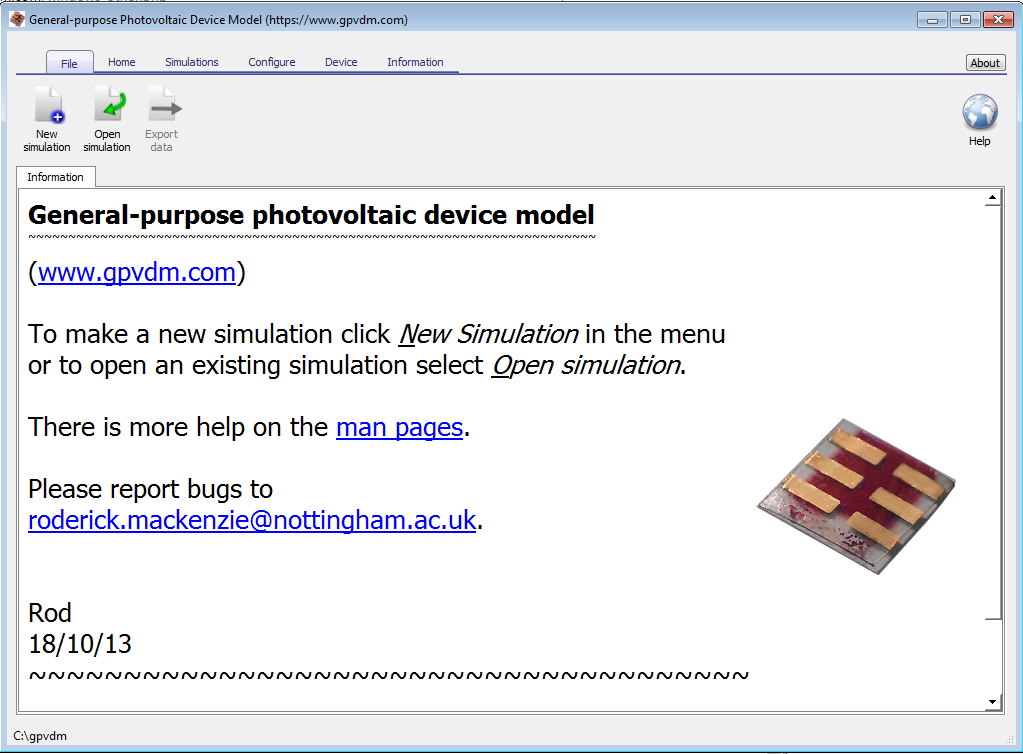
\includegraphics[width=100mm,height=70mm]{./images/new_open.png}
\caption{The main gpvdm simulation window.}
\label{fig:new_open}
\end{figure}

Click on the $new~simulation$ button.  This will bring up the new simulation window (see figure \ref{fig:new_new}).  From this window select the $Organic~Solar~Cell$ option and click next.  Gpvdm dumps a lot of data to disk, I therefore recommend you save the simulation to a local disk such as the C:\textbackslash drive, a network drive or usb stick drive will be far too slow for the simulation to run.  I would also not save the simulation onto OneDrive or Dropbox as they are also too slow and saving it there will generate a lot of network traffic.  If you are a power user doing a lot of fitting of experimental data I would also recommend (at your own risk(!)) disabling any extra antivirus software you have installed, as quite often the antivirus software can't keep up with the read/writes to disk.

\begin{figure}[H]
\centering
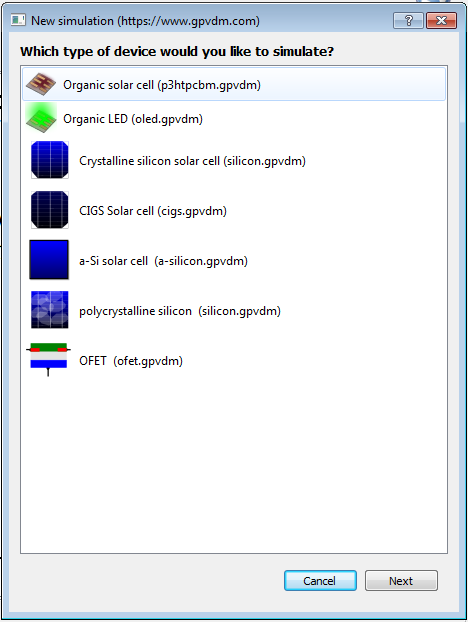
\includegraphics[width=100mm,height=70mm]{./images/new.png}
\caption{New simulation window}
\label{fig:new_new}
\end{figure}

Once you have saved the simulation, the main gpvdm simulation window will be brought up (see figure \ref{fig:simpleinterface}). You can look around the structure of the solar cell, by dragging the picture of the solar cell with your mouse.  Try pressing on the buttons beneath the red square, they will change the orientation to the \emph{xy}, \emph{yz} or \emph{xz} plane. Notice the x,y,z origin marker in the bottom left of the 3D window.  The icon with four squares will give you an orthographic view of the solar cell.


\begin{figure}[H]
\centering
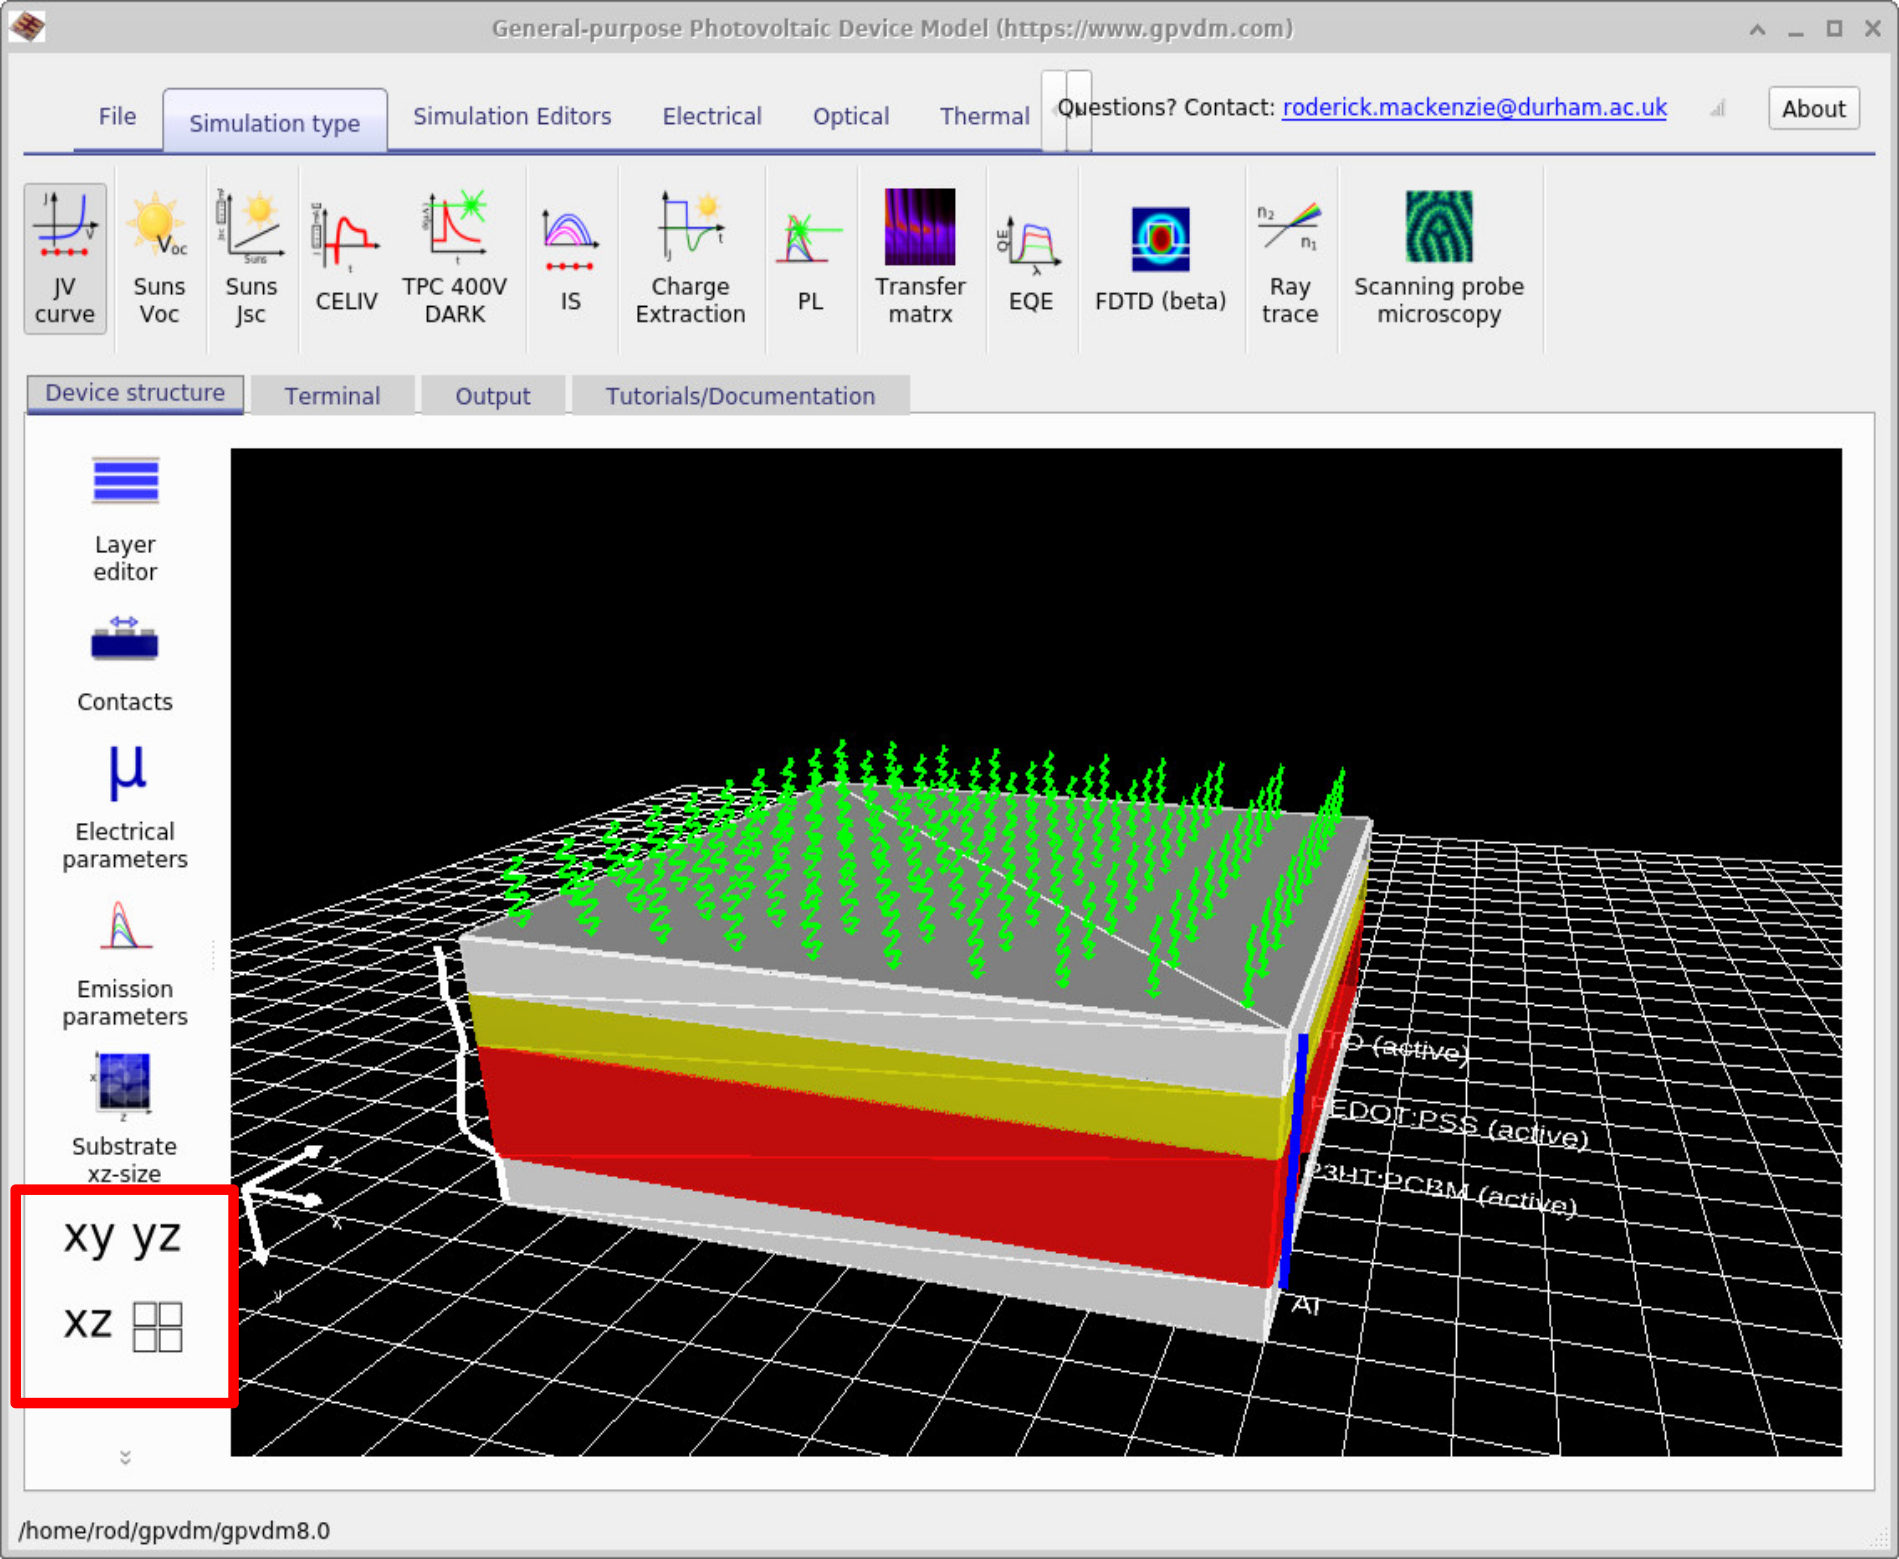
\includegraphics[width=100mm,height=70mm]{./images/simple_interface.png}
\caption{The main gpvdm simulation window}
\label{fig:simpleinterface}
\end{figure}

Click on the button called \emph{Run simulation} (hint it looks like a blue play button and is located in the \emph{file} one to the right of the "Simulation type ribbon" ).  This will run the simulation.  On slower computers it could take a while. Once the simulation is done, click on the $Output$ tab (see figure \ref{fig:output}), there you will see a list of files the simulation has written to disk.


\begin{figure}[H]
\centering
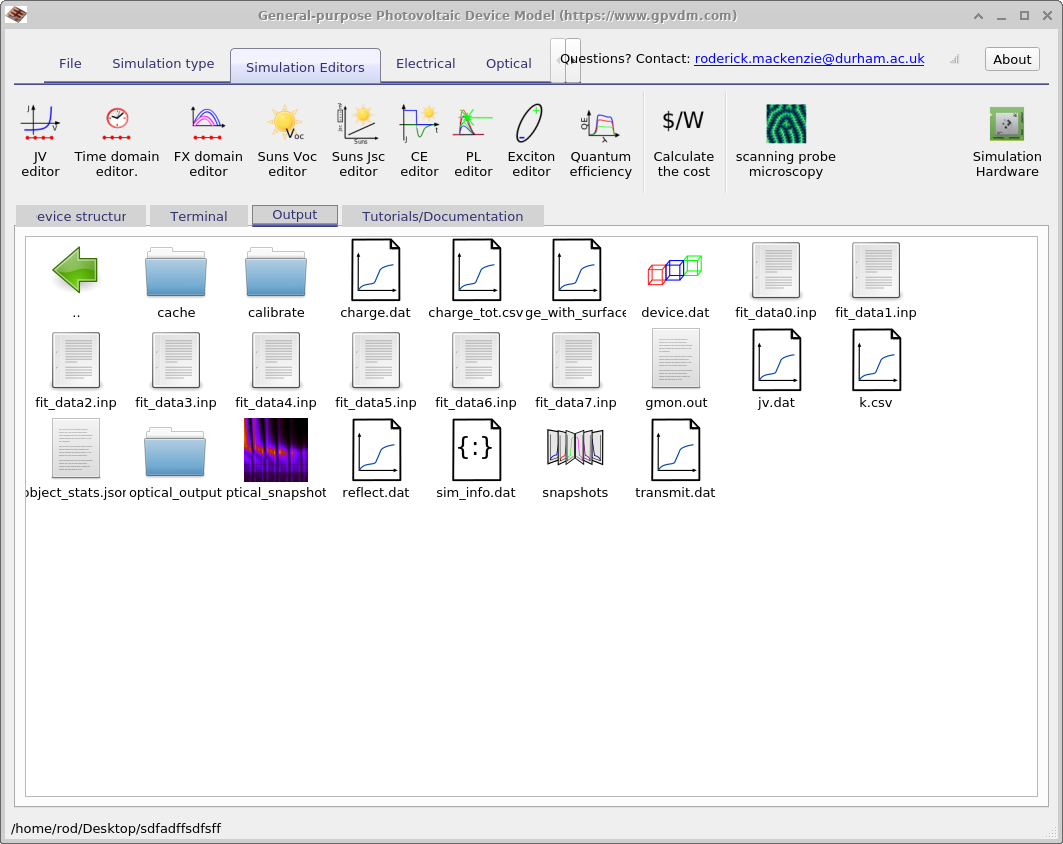
\includegraphics[width=100mm,height=70mm]{./images/output.png}
\caption{The \emph{Output} tab this is just like windows file explorer, you can explore the simulation directory tree.}
\label{fig:output}
\end{figure}

Key files the simulation produces are listed in the table below:

\begin{table}[H]
\begin{center}
\begin{tabular}{ |c|c|c| } 
 \hline
	File name 			& 	Description  \\ 
 \hline
	$jv.dat$ 			&	Current voltage curve \\ 
	$charge.dat$ 		&	voltage charge density\\ 
	$device.dat$ 		&	The 3D device model\\ 
	$fit_data*.inp$ 	&	Experimental fit data (for demo)\\
	$k.csv$ 			&	Recombination constant k\\ 
	$reflect.dat$ 		&	Optical reflection from device\\ 
	$transmit.dat$ 		&	Optical transition through device\\ 
	$snapshots$ 		&	Electrical snapshots see \ref{sec:snapshots}\\
	$optical\_snapshots$&	Optical snapshots see \ref{sec:snapshotsoptical} \\
	$sim\_info.dat$ 	&	Calculated $V_{oc}$, $J_{sc}$ etc.. see \ref{sec:siminfo}   \\
	$cache$ 			&	Cache see \ref{sec:cache}  \\
 \hline
\end{tabular}
\caption{Files produced by the JV simulation}
\label{fig:output}
\end{center}
\end{table}

Try opening $jv.dat$. This is a plot of the voltage applied to the solar cell against the current generated by the device.  These curves are also sometimes called the \emph{charistic diode curve}, we can tell a lot about the solar cell's performance by looking at these curves.  Hit the 'g' key to bring up a grid.

\begin{figure}[H]
\centering
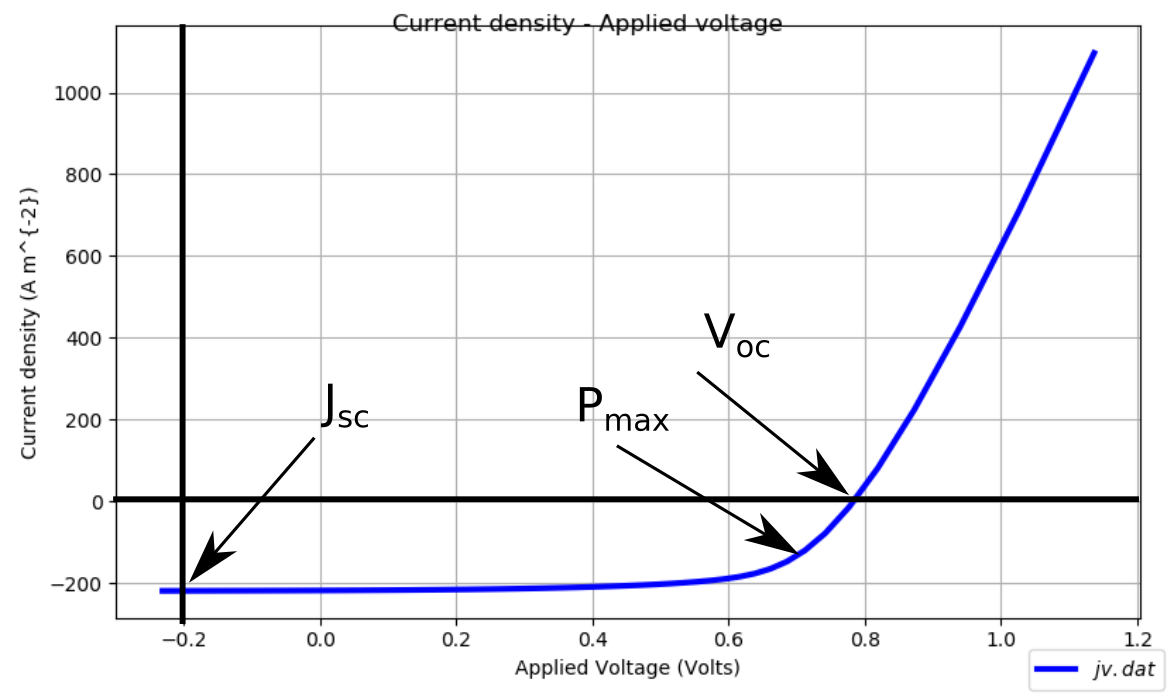
\includegraphics[width=100mm,height=70mm]{./images/jv_curve.png}
\caption{The output tab}
\label{fig:jv_curve}
\end{figure}


Now try opening up the file $sim\_info.dat$, this file displays information on the performance of the solar cell, such as the Open Circuit Voltage ($V_{oc}$ - the maximum Voltage the solar cell can produce when iluminated), efficiency ($\eta$ - the efficiency of the cell) , and short circuit current ($J_{sc}$ - the maximum current the cell can produce when it is illuminated).  Figure \ref{fig:jv_curve}, shows where you can find these values on the JV curve.  The $sim\_info.dat$ file contains a lot of other parameters, these are described in detail in section \ref{sec:siminfo}.

\newpage
\subsection{Editing device layers}
\label{sec:layereditor}
Any device in gpvdm consists of a series of layers (this is sometimes referred to as the epitaxy - this is a term which comes from inorganic semiconductors). The layer editor can be accessed from the main simulation window, under the \emph{device structure} tab. This is visible towards the top of figure \ref{fig:simpleinterface}, and the layer editor is visible in figure \ref{fig:layereditor}.



\begin{figure}[H]
\centering
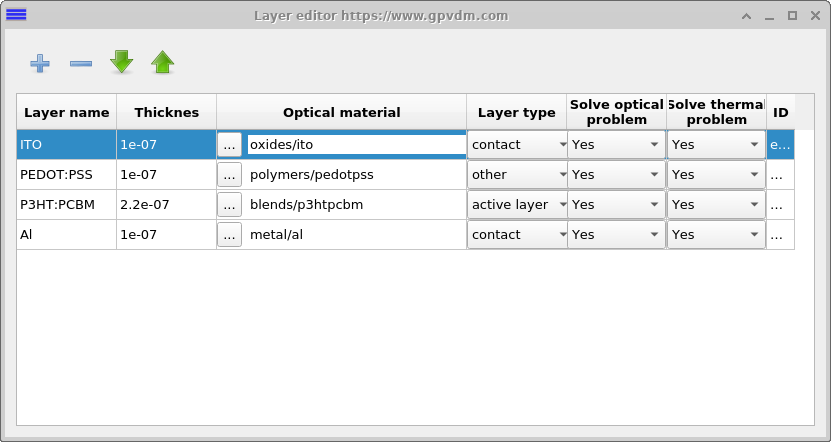
\includegraphics[width=100mm,height=70mm]{./images/layer_editor.png}
\caption{The layer editor window.}
\label{fig:layereditor}
\end{figure}

The layer editor has the following columns:

\begin{itemize}
  \item Layer name: Is the English name describing the layer. You can call your layers what you want (i.e. ITO, PEDOT, fred or bob) it has no physical meaning.
  \item Thickness: Is the layer thickness given in meters.
  \item Optical material: Specifies the n/k data which is used to describe the materials optical properties. In the simulation the n/k data are taken from experimental values stored in the optical database \ref{sec:materialdatabase} and have nothing to do with the electrical material properties such as effective band gap.
  \item Layer type: Specifies to the simulation how the layer is treated when performing a simulation. There are three types of layer
	\begin{itemize}
	  \item active: This type of layer is electrically active and the drift diffusion solver will solve the electrical equations in this layer type. See section \ref{sec:electrical}. You can have as many active layers as you like but they must be contiguous.
 	  \item contact: This tells the model that a layer is a contact and a voltage should be applied, see section \ref{sec:contacteditor} for more details.
 	  \item other: Any layer which is not a contact or active.

	\end{itemize}
\end{itemize}

%\vspace*{\fill}

\fbox{
\parbox{0.9\textwidth}{
\color{blue} Task \addtocounter{question}{1}\thequestion : Try varying the thickness of the P3HT:PCBM layer in 10 steps $100 nm$ to $500 nm$ each time you do this, run the simulation and make a note of the $V_{oc}$, Fill Factor and the $J_{sc}$ current.  Plot a graph of thickness v.s. these parameters. Which thickness is most efficient? 
}\par
}
\\

Which layers should be active?: A common mistake people make when starting to simulate devices is to try to make all the layers in their device active because their logic is: Current must be flowing through them so they must be active right?  However, in for example a solar cell only the BHJ or in a perovskite device the perovskite layer will have both species of carriers (electrons+holes) and complex effects such as photogeneration, recombination and carrier trapping. So in this layer it makes sense to solver the drift diffusion equations.  Other layers which don't have both species of carriers can be treated simple parasitic resistances see section \ref{sec:parasitic}. I would only recommend setting other layers of the device to active (such as the HTL/ETL) if you are trying to investigate effects such as s-shaped JV curves or devices which clearly need multiple active layers such as OLEDs. In general, try to minimize the number of active layers and always keep simulations as simple as possible to explain the physical effects you see.  

\newpage
\subsection{The contact editor}
\label{sec:contacteditor}
The contact editor is used to configure the electrical contacts.  Which layers act as contacts is configured in the layer editor see section \\ref{sec:layereditor}  The contact editor has the following fields:

\begin{figure}[H]
\centering
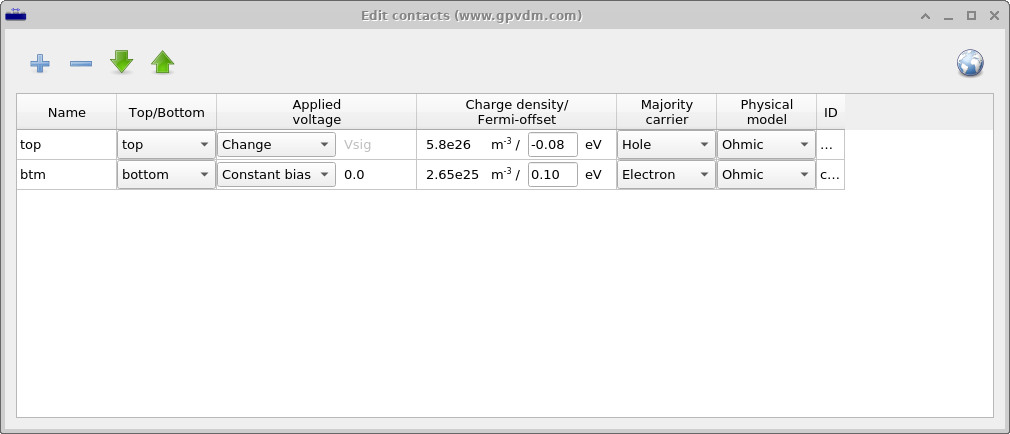
\includegraphics[width=100mm,height=70mm]{./images/contact_editor.png}
\caption{The contact editor}
\label{fig:contacteditor}
\end{figure}

\begin{itemize}
  \item Name: The name of the contact, this can be any English word. It has no physical meaning.
  \item Top/Bottom: Sets if the contact is on the top, bottom or in 2D simulation left and right of the device are also valid.
  \item Applied voltage: Sets the applied voltage on the contact. You first have to select what type of applied voltage you want:
		\begin{itemize}
		\item Ground: This will set the contact to zero volts i.e. ground. 0V is always taken as ground.
		\item Constant bias: This will apply a constant bias to a contact.  It can be set to zero, and would then be equivalent to ground.  In OFET simulations the voltage value can be set to bias one contact to a desired constant voltage.
		\item Change: If a contact is set to 'Change' this tells the simulation to apply a changing voltage to this contact. For example if you are performing a JV sweep, the sweep voltage will be applied to this contact.  Similarly if you are doing an IS simulation (TPV, TPC, ToF etc..) the voltage will be applied/measured to this contact.
		\end{itemize}
  \item Charge density: This sets the majority charge density on the contacts. The Fermi-offset is calculated from the charge density. The model does not use Fermi-offset as an input, it uses charge density.
  \item Majority carrier: This sets the majority carrier density to electrons or holes.
  \item Physical model: This selects if you have ohmic contacts or schottky contacts. I recommend using ohmic contacts.

\end{itemize}

\fbox{
\parbox{0.9\textwidth}{
\color{blue} Task \addtocounter{question}{1}\thequestion : For a good contact which results in a high efficiency device, the Fermi-offset will be exactly 0 eV or very small. Firstly set the Fermi-offset to zero for both contacts, and run a simulation.  What efficiency cell do you get? Now set the Fermi-offset to $0.3 eV$ what efficiency cell do you now have? Make a note of the charge densities on the contacts which these Fermi-offsets produce. 
}\par
}
\\

\newpage
\subsection{Parasitic elements}
\label{sec:parasitic}

Many devices have parasitic shunt and series resistances associated with them.  Shunt resistances ($R_{s}$) are caused by conduction straight through the device in thin novel devices this is often caused by impurities in the material system.  Parasitic series resistances ($R_{s}$) are often associated with the resistance of the contacts, the resistance of the HTL/ETL or any other resistances which are not associated with the active layer.  These resistance can be seen for a typical solar cell in figure \ref{fig:parasitic_circuit} also shown in the figure is the ideal diode of the device. These resistances can be set in the parasitic component window shown in figure \ref{fig:parasitic}


\begin{figure}[h!]
\centering
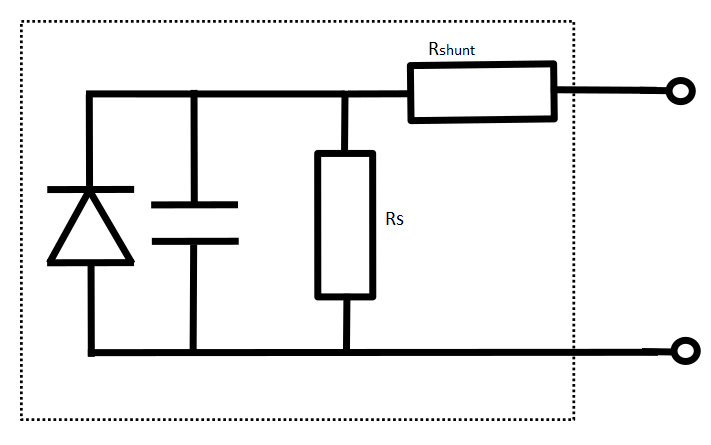
\includegraphics[width=100mm]{./images/parasitic_circuit.png}
\caption{Circuit model of a solar cell.}
\label{fig:parasitic_circuit}
\end{figure}


You can change the values of series and shunt resistance in gpvdm, by going to the \emph{Device structure} tab and then clicking on the \emph{Parasitic components} button.

\begin{figure}[H]
\centering
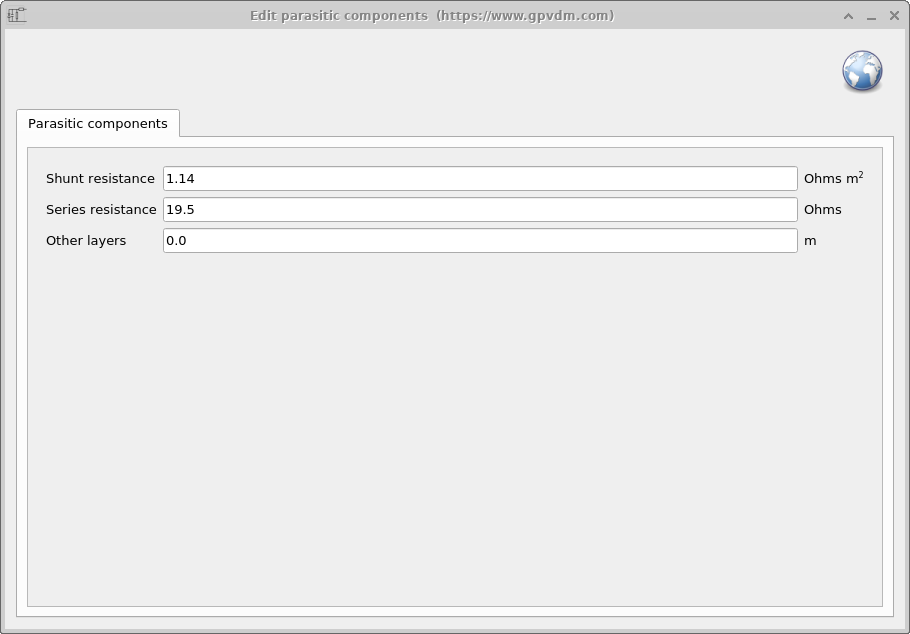
\includegraphics[width=100mm,height=70mm]{./images/parasitic.png}
\caption{The parasitic component editor}
\label{fig:parasitic}
\end{figure}

Due to the flat broad contacts on a solar cell, there is often a capacitance associated with the device, this is important for transient measurements and can be calculated with the equation:

\begin{equation}
C=\frac{\epsilon_r \epsilon_0 A}{d+\Delta}
\end{equation}

where $A$ is the area of the device $\epsilon$ are the hyperactivities, and $d$ is the thickness of the device.  Often for various reasons the measured capacitance of the device does not match what one would expect from the above equation. Therefore the term "Other layers" ($\Delta$) has been added to the parasitic window to account for differences between measured capacitance and layer measured layer thicknesses.

\fbox{
\parbox{0.9\textwidth}{
\color{blue} Task \addtocounter{question}{1}\thequestion : In the optical tab you will find a control called \emph{Light intensity}, this controls the amount of light which falls on the device in Suns.  Set it to zero so that the device is in the dark.  Then run two JV curve simulations, one with a shunt resistance of $1~Ohm~m^2$ and one with a shunt resistance of $1x10^{6}~Ohm~m^2$ (Hint you will have to enter $1e6$ in the text box).  What happens to the dark JV curve?  Now try running the same same simulations again but in the light.
}\par
}
\newpage
\subsection{Electrical parameters}
\label{sec:doseditor}
The electrical parameter editor enables you to change the electrical parameters associated with the active layers. Here you can change mobilities, trap constants etc.  The toolbar at the top of the window allows you to turn off and on various electrical mechanisms including:

\begin{itemize}
  \item Auger recombination: This switches on and off Auger recombination. See \ref{sec:auger} for more information.
  \item Dynamic SRH traps: This is used to turn on and off dynamic SRH traps.  See section \ref{sec:SRHintro} for more information.
  \item Equilibrium SRH traps: This can be used to introduce a single equilibrium trap level.  See section \ref{sec:SRHintro} for more information.
  \item Excitons: This enables the excition diffusion equation to be solved along with the electrical equations. See section \ref{sec:excitions} for more information.
\end{itemize}

\begin{figure}[H]
\centering
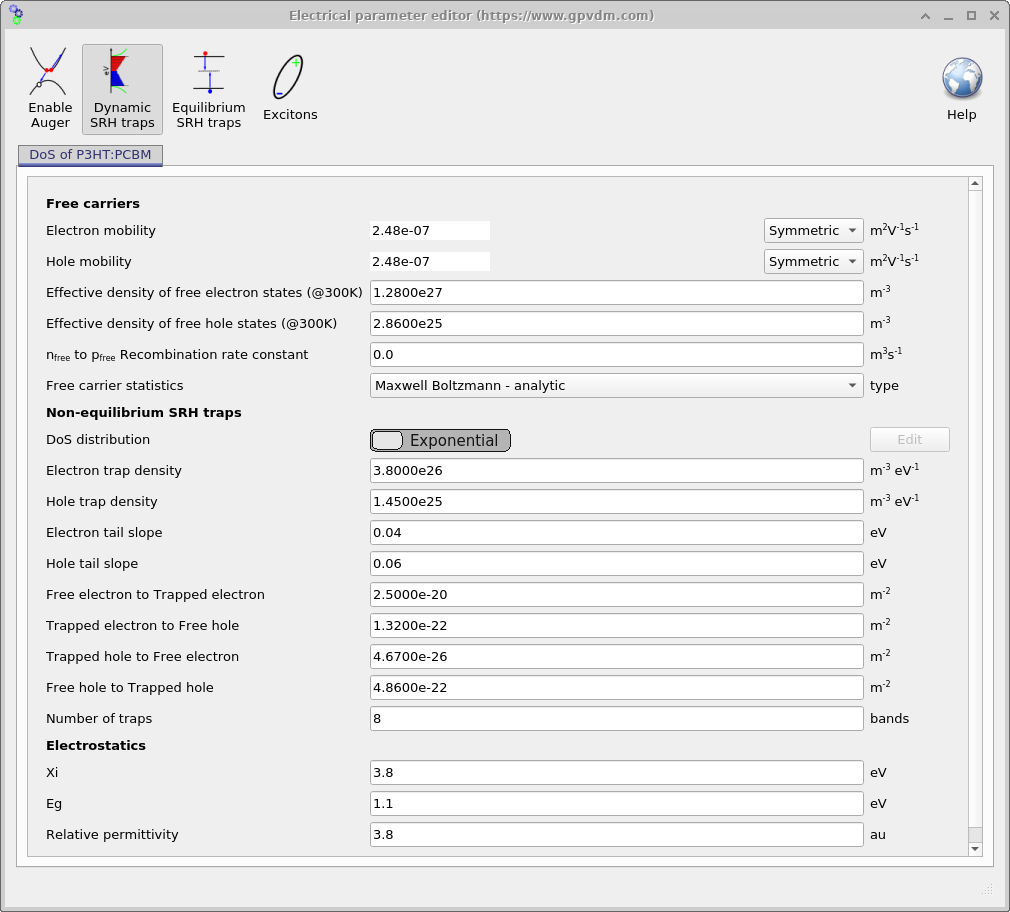
\includegraphics[width=100mm,height=70mm]{./images/dos_editor.png}
\caption{Electrical parameter window}
\label{fig:electricalparamwindow}
\end{figure}

\fbox{
\parbox{0.9\textwidth}{
\color{blue} Task \addtocounter{question}{1}\thequestion : The values of electron mobility dictate how easily charge can move in the device.  You can think of this value as akin to resistance or a sort of microscopic resistance. Try try increasing the mobilities by two orders of magnitude and look what happens to the light JV curve of the device and the efficiency, FF, $V_{oc}$ and $J_{sc}$  Do you think it is good to have a low or high value of mobility?
}\par
}
\\

\fbox{
\parbox{0.9\textwidth}{
\color{blue} Task \addtocounter{question}{1}\thequestion : Recombination is described later in detail but for now we can simply think of it as how many electrons and holes meet each other in a given time. As stated above there are various types of recombination which can happen in organic semiconductors, but for now we will \emph{just consider}  the case when a free electron meets a free hole.  This is sometimes called bi-molecular recombination, the equation for this is given by:
\begin{equation}
R(x)=kn(x)p(x)
\end{equation}
Where $n(x)$ is the density of electrons and $p(x)$ is the density of holes, and k is a rate constant.  Before trying to understand this rate, firstly turn off the more complex SRH recombination by clicking on the \emph{Dynamic SRH traps} in figure \ref{fig:electricalparamwindow}.  You will notice lots of text boxes disappear. Then try changing the value of $k$ which is set in the text box called $n_{free}$ to $p_{free}$ Recombination rate constant, from 1e-15 to 1e-20 in five steps.  Run a simulation each time you change the value and make a graph of the efficiency of the cell as you change the value. 
}\par
}
\\


